\documentclass[kulak]{kulakarticle} % options: kulak (default) or kul

\newcommand{\ud}{\mathrm{d}}  
\usepackage{subfigure}
\usepackage{amstext}
\usepackage{amsmath}


\title{Basic theory\\ VEM for 2D elastic mechanics problems}
\author{Bingbing Xu}
\date{Institute of Continuum Mechanics}
\address{
	\textbf{Bingbing Xu} \\
	bingbing.xu@ikm.uni-hannover.de}
\begin{document}

\maketitle

\section{Problem statement}
\label{r5.s1}
\subsection{Governing equation}
Considering the problems in solid mechanics defined in domain $\Omega\subseteq\mathbb{R}^d$ with boundary $\partial\Omega=\Gamma$($d$ is the dimension),
the strong form of the boundary value problem of elasticity is given by:

Find $\bm{u}(\bm{x}):\bar{\Omega}\rightarrow\mathbb{R}^d$ such that
\begin{subequations}
    \begin{equation}
        \nabla\cdot\bm{\sigma}+\bm{f} = 0,\quad \bm{x}\in\Omega,
    \end{equation}
    \begin{equation}
        \bm{u}=\bm{u}_D,\quad\bm{x} \in\Gamma_{D},
    \end{equation}
    \begin{equation}
        \bm{\sigma}\cdot\bm{n}_N = \bar{\bm{t}},\quad\bm{x}\in\Gamma_{N}.
    \end{equation}
\end{subequations}

The Cauchy stress tensor $\bm{\sigma}$ follows Hooke's low 
\begin{equation}
    \bm{\sigma} = \bm{C}\bm{\varepsilon},
\end{equation}
where 
\begin{equation}
    \bm{\varepsilon} = \frac{1}{2}\left(\nabla\bm{u}+\nabla\bm{u}^T\right).
\end{equation}

\subsection{Continuous variation problem}
\label{r5.s1.2}
Assuming 
\begin{equation}
    \bm{\mathcal{V}} = \left\{\bm{v}\in H^1(\Omega)^d:\bm{v} = \bm{0}\quad \text{on}\quad \Gamma_0\right\},
\end{equation}
the weak form of the governing equation is: 
find $\bm{u}\in\bm{\mathcal{V}}$ such that 
\begin{equation}
    \int_\Omega-\frac{\partial\sigma_{ij}(\bm{u})}{\partial x_j}v_i\ud\Omega = \int_\Omega f_iv_i\ud\Omega.
\end{equation}
By using integration by parts, we have
\begin{equation}
    -\int_{\partial\Omega}\sigma_{ij}(\bm{u})v_in_j\ud\Gamma+\int_\Omega\sigma_{ij}(\bm{u})\frac{\partial v_i}{\partial x_j}\ud\Omega = \int_{\Omega}f_iv_i\ud\Omega.
\end{equation}

Considering the symmetry of stress tension, we have
\begin{equation}
    \sigma_{ij}(\bm{u})\frac{\partial v_i}{\partial x_j} = \sigma_{ij}(\bm{u})\frac{1}{2}\left(\frac{\partial v_i}{\partial x_j}+\frac{\partial v_j}{\partial x_i}\right)
    =\sigma_{ij}(\bm{u})\varepsilon_{ij}(\bm{v}),
\end{equation}
and the last form can be written as 
\begin{equation}
    \label{r5.s1.2.bilinear1}
    \int_\Omega\sigma_{ij}(\bm{u})\varepsilon_{ij}(\bm{v})\ud\Omega = \int_\Omega f_iv_i\ud\Omega+\int_{\Gamma_N}\bar{t}_iv_i\ud\Gamma,
\end{equation}
or the matrix form as 
\begin{equation}
    \label{r5.s1.2.bilinear2}
    \int_\Omega\bm{\sigma}(\bm{u}):\bm{\varepsilon}(\bm{v})\ud\Omega = \int_\Omega\bm{f}\cdot\bm{v}\ud\Omega+\int_{\Gamma_N}\bar{\bm{t}}\cdot\bm{v}\ud\Gamma.
\end{equation}
Then the variation problem can be written as:
find $\bm{u}\in\bm{\mathcal{V}}$ such that 
\begin{equation}
    \label{r5.s1.variationBilinear}
    a(\bm{u},\bm{v}) = L (\bm{v}),\bm{v}\in\bm{\mathcal{V}},
\end{equation}
where 
\begin{equation}
    a(\bm{u},\bm{v}) = \int_\Omega\bm{\sigma}(\bm{u}):\bm{\varepsilon}(\bm{v})\ud\Omega,
\end{equation}
\begin{equation}
    L (\bm{v}) = \int_\Omega\bm{f}\cdot\bm{v}\ud\Omega+\int_{\Gamma_N}\bar{\bm{t}}\cdot\bm{v}\ud\Gamma.
\end{equation}

\subsection{Mathematical preliminaries}
\label{r5.s1.3}
It is more convenient to reduce the tensor expressions into equivalent matrix and vector representations. 
In particular, for any symmetric $2\times 2$ matrix $\bm{A}$, denote its Voigt representation $\bar{\bm{A}}$ by 
\begin{equation}
    \bm{A} = \begin{bmatrix}
        a_{11} & a_{12} \\ a_{21} & a_{22}
    \end{bmatrix},\quad 
    \bar{\bm{A}} = \begin{Bmatrix}
        a_{11} \\ a_{22} \\ a_{12}
    \end{Bmatrix}.
\end{equation}

On using Voigt (engineering) notation, we can write the stress and strain in terms of $3\times 1$ arrays:
\begin{equation}
    \bar{\bm{\sigma}} = \begin{Bmatrix}
        \sigma_{11} \\ \sigma_{22} \\ \sigma_{12}
    \end{Bmatrix},\quad 
    \bar{\bm{\varepsilon}} = \begin{Bmatrix}
        \varepsilon_{11}\\ \varepsilon_{22} \\ 2\varepsilon_{12}
    \end{Bmatrix}.
\end{equation}

Furthermore, by using these conventions we can also express the strain-
displacement relation and the constitutive law in matrix form as:
\begin{equation}
    \bar{\bm{\sigma}} = \bm{C}\bar{\bm{\varepsilon}},\quad 
    \bar{\bm{\varepsilon}} = \bm{S}\bm{u},
\end{equation}
where $\bm{S}$ is a matrix differential operator that is given by
\begin{equation}
    \bm{S} = \begin{bmatrix}
        \frac{\partial}{\partial x} & 0 \\
        0 & \frac{\partial}{\partial y} \\
        \frac{\partial}{\partial y} & \frac{\partial}{\partial x}
    \end{bmatrix},
\end{equation}
and $\bm{C}$ is the associated matrix representation of the material tensor that
is given by 
\begin{equation}
    \bm{C} = \frac{E}{(1-\nu^2)}\begin{bmatrix}
        1 & \nu & 0\\
        \nu & 1 & 0\\
        0 & 0 & \frac{1-\nu}{2}
    \end{bmatrix},
\end{equation}
for plane stress and 
\begin{equation}
    \bm{C} = \frac{E}{(1+\nu)(1-2\nu)}\begin{bmatrix}
        1-\nu & \nu & 0\\
        \nu & 1-\nu & 0\\
        0 & 0 & \frac{1-2\nu}{2}
    \end{bmatrix},
\end{equation}
for plane strain.
Besides, $E$ is Young's modulus and $\nu$ of the Poisson's ratio of the material.

\section{Projection operator of the displacement-for strain}
\label{r5.s2}
\subsection{Projection operator}
The projection is designed as 
\begin{equation}
    \Pi_{E,k}:\bm{\mathcal{V}}^h(E)\rightarrow\bm{\mathcal{P}}_k(E),\quad \bm{\mathcal{V}}^h(E)\equiv \left[\mathcal{V}^h(E)\right]^2.
\end{equation}
The operator is constructed locally in each polygon so that satisfies the following orthogonality condition 
\begin{equation}
    a_E\left(\bm{v}^h-\Pi_k\bm{v}^h,\bm{p}\right) = 0.
\end{equation}

The basis functions for space $\bm{\mathcal{P}}_k$ are selected as 
\begin{itemize}
    \item $k=0$:
    \begin{equation}
        \bm{m}_0 =
        \begin{pmatrix}
            1 \\ 0
        \end{pmatrix},
        \begin{pmatrix}
            0\\1
        \end{pmatrix};
    \end{equation}
    \item $k=1$:
    \begin{equation}
        \bm{m}_1 =\bm{m}_0,
        \begin{pmatrix}
            -\eta \\ \xi
        \end{pmatrix},
        \begin{pmatrix}
            \eta \\ \xi
        \end{pmatrix},
        \begin{pmatrix}
            \xi \\ 0
        \end{pmatrix},
        \begin{pmatrix}
            0 \\ \eta
        \end{pmatrix},
    \end{equation}
\end{itemize}
where 
\begin{equation}
    \xi = \frac{x-x_E}{h_E},\quad \eta = \frac{y-y_E}{h_E},
\end{equation}
and $(x_E,y_E)$ is the center of the element and $h_E$ is the characteristic length of the element.


The definition of the local projection operator $\Pi_k\equiv \Pi_{E,k}$ can be rewritten as 
\begin{equation}
    a_E(\bm{v}^h,\bm{p}) = a_E\left(\Pi_k\bm{v}^h,\bm{p}\right),\quad\forall \bm{p}\in\bm{\mathcal{P}}_k(E).
\end{equation}
Furthermore, coefficients of the projection of shape functions are determined due to the orthogonal property
\begin{equation}
    \begin{aligned}
        \int_E\bm{\varepsilon}(\bm{m})\bm{C}\bm{\varepsilon}(\bm{\phi}^T)\ud\Omega &= \int_E\bm{\varepsilon}(\bm{m})\bm{C}\bm{\varepsilon}(\bm{\phi}^T\bm{\Pi})\ud\Omega \\ &=
        \int_E\bm{\varepsilon}(\bm{m})\bm{C}\bm{\varepsilon}(\bm{m}^T\bm{\Pi}_k^*)\ud\Omega \\ &= \int_E\bm{\varepsilon}(\bm{m})\bm{C}\bm{\varepsilon}(\bm{m}^T)\ud\Omega\bm{\Pi}_k^*
    \end{aligned}
\end{equation}
or
\begin{equation}
    a_E\left(\bm{m},\bm{\phi}^T\right) = a_E\left(\bm{m},\bm{\phi}^T\bm{\Pi}_k\right) = a_E\left(\bm{m},\bm{m}^T\bm{\Pi}_k^*\right) = a_E\left(\bm{m},\bm{m}^T\right)\bm{\Pi}_k^*.
\end{equation}

Lastly, the matrix of the projection operator can be written as 
\begin{equation}
    \label{r5.s2.projection1}
    \left\{
        \begin{aligned}
            &\bm{G}\bm{\Pi}_k^* = \bm{B}\\
            &\text{constraints}
        \end{aligned}
    \right.,
\end{equation}
where 
\begin{equation}
    \label{r5.s2.G}
    \bm{G} = a_E\left(\bm{m},\bm{m}^T\right) = \int_E\bm{\varepsilon}(\bm{m})\bm{C}\bm{\varepsilon}(\bm{m}^T)\ud\Omega,
\end{equation}
\begin{equation}
    \label{r4.s2.B}
    \bm{B} = a_E\left(\bm{m},\bm{\phi}^T\right) = \int_E\bm{\varepsilon}(\bm{m})\bm{C}\bm{\varepsilon}(\bm{\phi}^T)\ud\Omega,
\end{equation}
and 
\begin{equation}
    \bm{G} = \bm{B}\bm{D},\quad\bm{\Pi}_k = \bm{D}\bm{\Pi}_k^{*},
\end{equation}
where 
\begin{equation}
    \bm{D}_{j\alpha} = \text{dof}_j(\bm{m}_\alpha).
\end{equation}

The matrix $\bm{B}$ can be calculated by 
\begin{equation}
    \begin{aligned}
        \bm{B} &= \int_E\bm{\varepsilon}(\bm{m})\bm{C}\bm{\varepsilon}(\bm{\phi}^T)\ud\Omega\\
        &=-\int_E\nabla\cdot\left(\bm{C}\bm{\varepsilon}(\bm{m})\right)\cdot\bm{\phi}^T\ud\Omega+
        \int_{\partial E}\bm{\varepsilon}(\bm{m})\bm{C}\bm{n}\bm{\phi}^T\ud\Gamma,
    \end{aligned}
\end{equation}
where the first term is zero and  
\begin{equation}
    \bm{n} = \begin{bmatrix}
        n_x & 0\\ 0 & n_y\\ n_y & n_x
    \end{bmatrix}.
\end{equation}

As mentioned in Eq.\eqref{r5.s2.projection1}, the constraints should be introduced as 
\begin{equation}
    \label{r5.s2.constraint}
    \left\{
        \begin{aligned}
            &\int_{E}\nabla\times\Pi_k^1\bm{v}\ud\Omega = \int_E\nabla\times\bm{v}\ud\Omega\\
            &\int_{\partial E}\Pi_k^1\bm{v}\ud\Gamma = \int_{\partial E}\bm{v}\ud\Gamma
        \end{aligned}
    \right.,
\end{equation}
where 
\begin{equation}
    \int_E\nabla\times\bm{v}\ud\Omega = \int_{\partial E}\bm{v}\cdot\bm{t}_e\ud\Gamma,
\end{equation}
where 
\begin{equation}
    \bm{t}_e = [-n_y,n_x]^T.
\end{equation}

For the first term in Eq.\eqref{r5.s2.constraint}, the right hand can be written as 
\begin{equation}
    \int_{E}\nabla\times\bm{\phi}^T\ud\Omega = \int_{\partial E}\bm{t}_e^T\bm{\phi}^T\ud\Gamma =
    \int_{\partial E}
    \begin{bmatrix}
        -n_y & n_x
    \end{bmatrix}
    \begin{bmatrix}
        \phi^T & \\ & \phi^T
    \end{bmatrix}
    \ud\Gamma.
\end{equation}

For the second term in Eq.\eqref{r5.s2.constraint}, we have 
\begin{equation}
    \int_{\partial E}\bm{\phi}^T\ud\Gamma = 
    \int_{\partial E}
    \begin{bmatrix}
        \phi^T & \\ & \phi^T
    \end{bmatrix}
    \ud\Gamma.
\end{equation}

Lastly, we have 
\begin{equation}
    \tilde{\bm{G}} = \tilde{\bm{B}}\bm{D},
\end{equation}
and the projection can be obtained as 
\begin{equation}
    \bm{\Pi}_k^* = \tilde{\bm{G}}^{-1}\tilde{\bm{B}},\quad \bm{\Pi}_k = \bm{D}\bm{\Pi}_k^* = \bm{D}\tilde{\bm{G}}^{-1}\tilde{\bm{B}}.
\end{equation}


\subsection{Element stiffness matrix}
\label{r5.s2.2}
The stiffness matrix is obtained by the contributions of consistency and stability components
\begin{equation}
    \begin{aligned}
        \bm{K}_E &= \int_E\bm{\varepsilon}\left(\Pi\bm{\phi}\right)\bm{C}\bm{\varepsilon}\left(\Pi\bm{\phi}^T\right) \ud\Omega+\bm{K}_E^s\\
        &=\int_{\Omega}\bm{\Pi}^{*T}_k\bm{\varepsilon}(\bm{m})\bm{C}\bm{\varepsilon}\left(\bm{m}^T\right)\bm{\Pi}^*_k\ud\Omega+\bm{K}_E^s\\
        &=\bm{\Pi}^{*T}_k\int_{\Omega}\bm{\varepsilon}(\bm{m})\bm{C}\bm{\varepsilon}\left(\bm{m}^T\right)\ud\Omega\bm{\Pi}^*_k+\bm{K}_E^s\\
        &=\bm{\Pi}^{*T}_k\bm{G}\bm{\Pi}^*_k+\bm{K}_E^s,
    \end{aligned}
\end{equation}
and the stability component $\bm{K}_E^s$ can be selected as 
\begin{equation}
    \bm{K}_E^s = \tau^h\text{tr}\left(\bm{K}_E^c\right)\left(\bm{I}-\bm{\Pi}_k\right)^T\left(\bm{I}-\bm{\Pi}_k\right).
\end{equation}

\subsection{Numerical example}
% \begin{figure}[htbp]
% 	\centering
% 	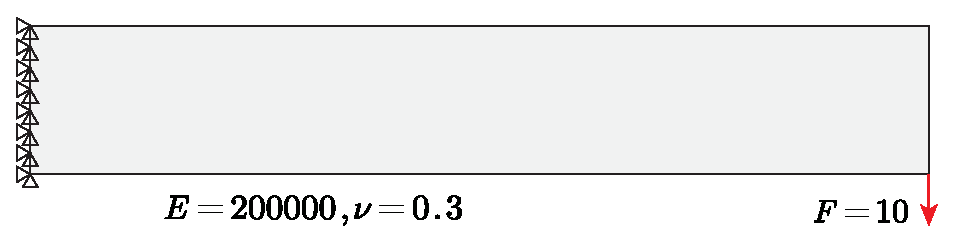
\includegraphics[width=10cm]{r4_s7_exam1Model.eps}
% 	\caption{The two-dimensional plane strain problem.}
% 	\label{r5.s2.f1}
% \end{figure}

\begin{figure}[htbp]
	\centering
	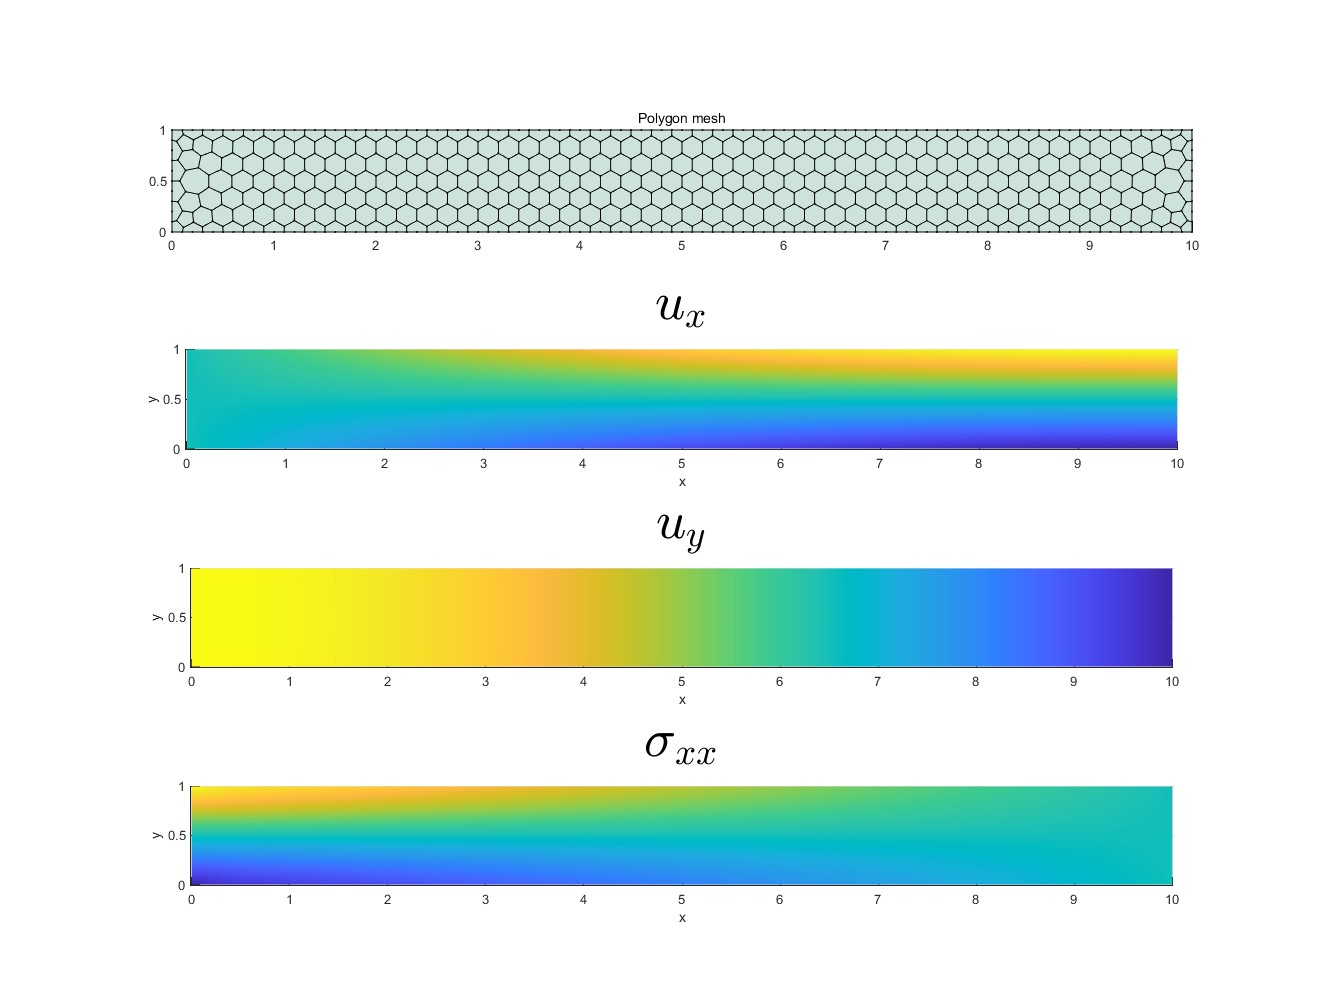
\includegraphics[width=10cm]{r5_s2_exam1C.jpg}
	\caption{Numerical solutions obtained by VEM.}
	\label{r5.s2.f2}
\end{figure}





% \newpage

% \begin{thebibliography}{99}
%     \bibitem{ref1} Alvin Chen, N. Sukumar, Stabilization-free virtual element method for plane elasticity, Computers \& Mathematics with Applications, 138:88-105, 2023.
%     \bibitem{ref2} B. Zhang, J. Zhao, Y. Yang, and S. Chen. The nonconforming virtual element method for elasticity problems. J. Comput. Phys., 378:394–410, 2019.
%     \bibitem{ref3} Mengolini, M., Benedetto, M. F., and Aragon, A. M. An engineering perspective to the virtual element method and its interplay with the standard finite element method. Computer Methods in Applied Mechanics and Engineering, 350, 995-1023.
% \end{thebibliography}


\end{document}
